\documentclass[11pt]{article}
\usepackage{enumerate}
\usepackage{fancyhdr}
\usepackage{amsmath}
\usepackage{graphicx}

\thispagestyle{empty}
\setlength{\parindent}{0cm}
\setlength{\parskip}{0.3cm plus4mm minus3mm}
\oddsidemargin = 0.0in
\textwidth = 6.5 in
\textheight = 9 in
\headsep = 0in

\title{CSCI 4100 Fall 2018 \\
% enter assignment number
Assignment 9 Answers}
\author{Damin Xu\\661679187}



\begin{document}
\maketitle
% enter question #
\noindent{\bf Problem 1}\\
Dimension of Z after 8th order transformation is 300*45.
\\\\
\noindent{\bf Problem 2}
\begin{figure}[htb] 
	{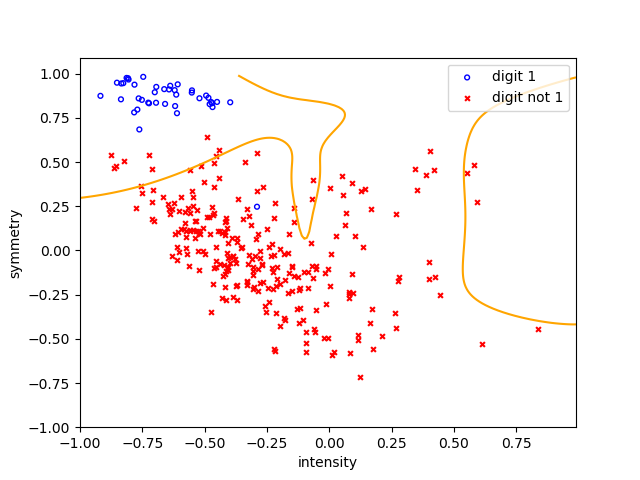
\includegraphics[height=7cm]{problem2.png}}
\end{figure}
\\There is overfitting.
\newpage
\noindent{\bf Problem 3}
\begin{figure}[htb] 
	{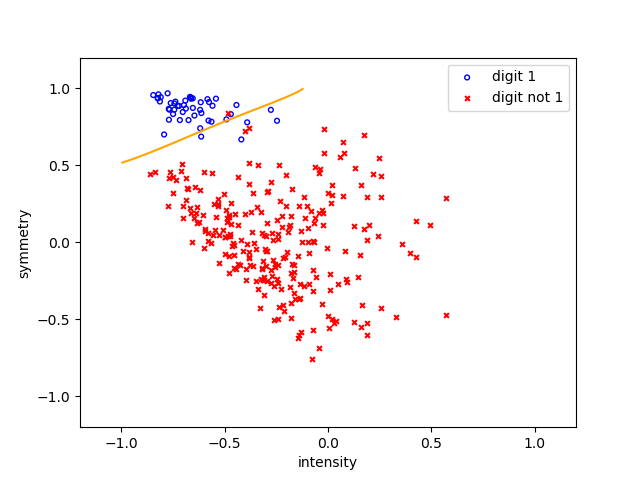
\includegraphics[height=7cm]{problem3.png}}
\end{figure}\\
There is underfitting.
\\\\
\noindent{\bf Problem 4}
\begin{figure}[htb] 
	{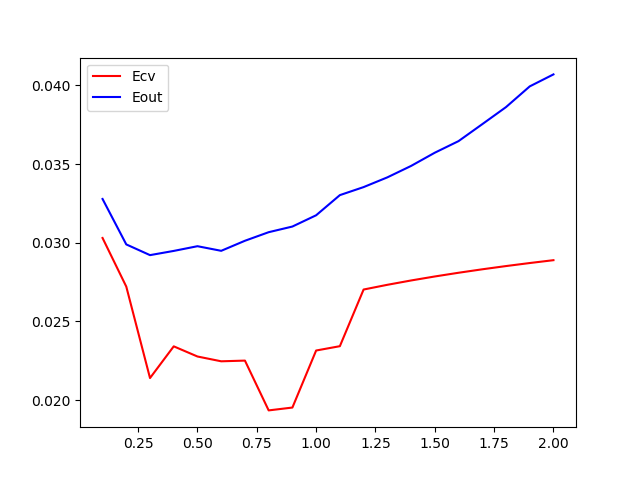
\includegraphics[height=7cm]{problem4.png}}
\end{figure}
\\When $E_{CV}$ is at the minimum, $E_{test}$ is almost at the minimum. So $E_{CV}$ indicates the best $\lambda$ which causes a relatively very small Etest.
\newpage
\noindent{\bf Problem 5}\\
\begin{figure}[htb] 
	{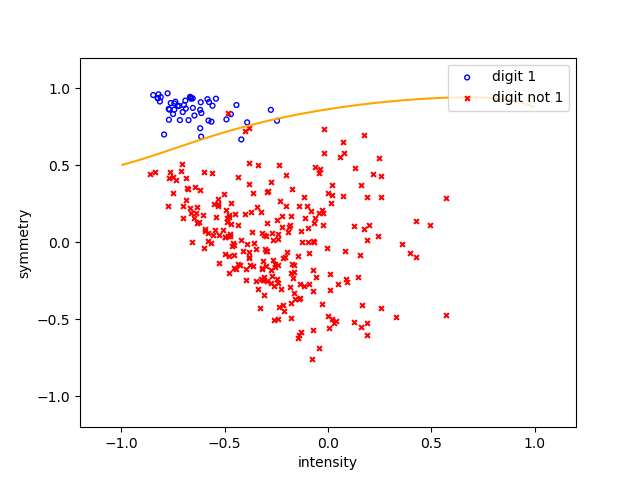
\includegraphics[height=7cm]{problem5.png}}
\end{figure}
\\The best $\lambda$ is 0.8.
\\\\
\noindent{\bf Problem 6}\\
The estimate $E_{out} = 0.030669072830919387 + 0.00248 = 0.0331$.
\\\\
\noindent{\bf Problem 7}\\
$E_{CV}$ is a biased estimate of $E_{test}$, because $\lambda^*$ is chosen from a range of $\lambda$ by test among the train set of 300 data, which means this $E_{CV}$ is close to $E_{in}$. Since $E_{in}$ is not unbiased, $E_{CV}$ is also unbiased.
\\\\
\noindent{\bf Problem 8}\\
$E_{test}(w_{reg}(\lambda^*))$ is a biased estimate of $E_{out}(w_{reg}(\lambda^*))$, because here the train set of data is randomly chosen from all data, this random chosen set may contain some bad data which cannot be classified well. The process of random pick continues until a better result is given. This causes data snopping.\\
\\
To fix this probelm, I would like to do the normalization after spliting train set from test set.
\end{document}
\end{document}
